\chapter{Evaluation}
\label{chap:evaluation}

This chapter discusses the strategies that were adopted in order to assess the fulfillment the objectives defined in \Cref{sec:objectives} were satisfied by the implemented solution;
%
Primarily, the chosen techniques were:
%
\begin{itemize}
    \item \textbf{unit tests}, that verify the functional aspects of the project and define a formalization of the expectations about the semantics;
    \item \textbf{empirical tests}, which consist of \textit{sample programs} run via simulation, in order to assess qualitative properties of the prototype.
\end{itemize}

\section{Unit testing}

In order to certify the correctness of the code written during development, the project was equipped with a suite of \textit{unit tests} of the implementation of the semantics.
%
Not only did this allow refactoring with greater confidence, but it also constituted a formalization of the expectations about the API of the language that is \textit{verifiable} and \textit{reproducible}.

In practice, unit tests were written using the \textit{ScalaTest}~\footnote{\url{https://www.scalatest.org/}} framework, one of the de facto standards for automated testing in Scala.
%
Out of the many testing styles that it offers, the chosen one was the \textit{FlatSpec}, due to its simple structure that promotes a behavior-driven approach to writing tests.

The most relevant tests that are included in the project are written for the \texttt{Semantics} trait.
%
The starting point of the process was to implement a mocked version of the incarnation and the related context, in order to both have access to the constructs of the language and to be able to manually trigger state changes for the flows to react to.
%
Being based on the same ideas as the \texttt{SimulationIncarnation}, the source code for the \texttt{MockIncarnation} is omitted.
%
As an example of the principles that guided this process, \Cref{lst:semantics-tests} shows a portion of the \texttt{SemanticsTests} class that includes tests for the \texttt{lift} construct.
%
\lstinputlisting[
    float,
    language=scala,
    caption={A portion of the \texttt{SemanticsTests} class including tests for the \texttt{lift} construct.},
    label={lst:semantics-tests},
]{listings/SemanticsTests.scala}
%
Typically, unit tests are implemented by constructing a flow that includes the primitive that is being tested, running it with an empty path using the given context implicitly, and then sampling the exports, possibly after notifying some state change.
%
The results of sampling are then asserted against some condition to verify that exports behave as expected.

\section{Sample programs}

While unit tests ensure the correctness of the semantics from a purely functional standpoint, they are not enough evaluate the overall behavior of the library and the complete fulfillment of the objectives.
%
To this purpose, a series of sample aggregate programs, for which the expected outcome is known in advance, was developed.

\Cref{lst:gradient-with-obstacles} shows the implementation of a comprehensive sample that showcases almost every feature of the language, i.e., a \textit{gradient with obstacles}.
%
The environment used by this sample is a 5x5 grid, where each device is a neighbor of the nearest device in each horizontal and vertical direction (\Cref{fig:gradient-environment}).
%
In addition, the device with ID $0$ is a source node, while devices $2$, $7$, and $12$ are obstacles.
%
\begin{figure}
    \centering
    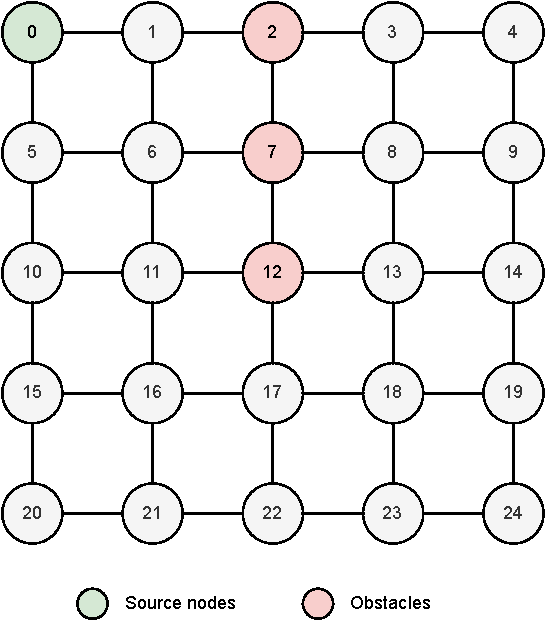
\includegraphics[width=0.5\textwidth]{figures/samples/gradient-environment.pdf}
    \caption{The reference environment for the gradient with obstacles.}
    \label{fig:gradient-environment}
\end{figure}
%
\lstinputlisting[
    float,
    language=scala,
    caption={A sample aggregate program computing a gradient with obstacles.},
    label={lst:gradient-with-obstacles},
]{listings/GradientSample.scala}

The gradient with obstacles sample can be built starting from a simple \textit{gradient}, thanks to the compositionality of aggregate computing.
%
The implementation of the gradient itself is just an adaptation of the one that is already known in the literature and from field calculus to the new API.
%
On top of that, obstacles are introduced by branching using the \texttt{obstacle} sensor provided by the incarnation, using a default constant flow with value $-1$ where and when the sensor evaluates to true.

Notice that, when the sample is run, the application stops logging after a certain amount of time, indicating that no more exports are being generated.
%
This demonstrates that the objective of \quotes{broadcasting messages only upon relevant changes} (recall \Cref{sec:objectives}) was fulfilled.
%
In addition, by looking at the last export of each device, the global field that is produced is shown in \Cref{fig:gradient-result}, which is the expected result.
%
\begin{figure}
    \centering
    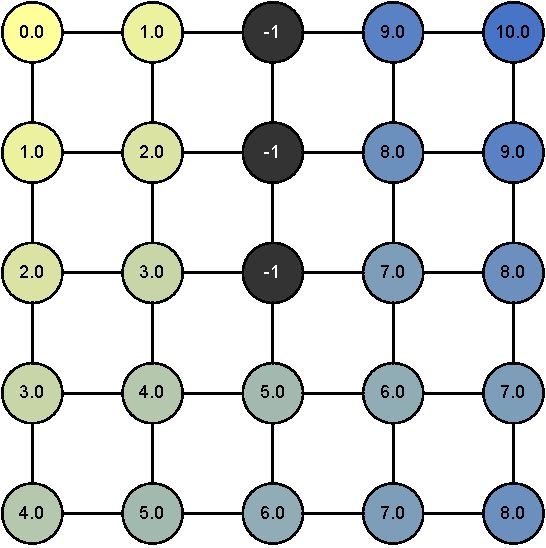
\includegraphics[width=0.5\textwidth]{figures/samples/gradient-result.pdf}
    \caption{The output field of the gradient with obstacles sample, after stabilization.}
    \label{fig:gradient-result}
\end{figure}

To prove that also the \quotes{compute only upon relevant changes} objective was satisfied, a small addition to the sample was introduced.
%
In fact, by placing these lines at the end of the \texttt{gradientSample()} method
%
\begin{lstlisting}[frame=single, language=scala]
Thread.sleep(5000)
sourcesSink.set(Set(4))
Thread.sleep(5000)
obstaclesSink.update(_ + 17)
\end{lstlisting}
%
the following behavior is exhibited:
%
\begin{itemize}
  \item initially, the gradient is computed normally, and it self-stabilizes in less than 5 seconds, with the same output as the previous configuration;
  \item after 5 seconds from the start of the simulation, the aggregate of devices recognizes a change in the source field and re-adapts itself in a reactive way;
  \item after 10 seconds, a new obstacle is detected by the network and the gradient adapts yet again.
\end{itemize}
%
Notice that, in this last scenario, updates do not reach portions of the network that are not influenced by the gradient change, implying that only computations that are strictly required are actually carried out.

For what concerns the last objective, i.e., \quotes{avoid re-evaluation of unaffected sub-computations}, another sample was created from scratch (\Cref{lst:test-re-evaluation}).
%
This program starts a simulation on a single device with a flow that branches on the \texttt{source} sensor, where the \quotes{then} branch performs some intense computation on a constant flow.
%
Subsequently, it changes the value of the source sensor back and forth in order to switch the selected branch alternatively.
%
In ScaFi, the intense computation would be re-evaluated on each round where the value of \texttt{source} was true.
%
To verify that this is not the case for this implementation, \texttt{someIntenseComputation} performs a side effect that prints to the console some text.
%
This is, indeed, a violation of the principles of referential transparency of functions passed to the constructs of the language, but it serves the purpose of counting the number of calls that are made to that method.
%
In fact, running this program results in \quotes{\textit{Doing some intense computation...}} being printed only once, while the device broadcasts messages five times instead, demonstrating that sub-computations that are not affected by changes in the environment are not re-evaluated.
%
\lstinputlisting[
    float,
    language=scala,
    caption={A sample aggregate program verifying that sub-computations do not get re-evaluated if their dependencies do not change.},
    label={lst:test-re-evaluation},
]{listings/TestReEvaluation.scala}

% Finally, the usability of the core API of the language can be rated by comparing the versions of the gradient written with ScaFi (recall \Cref{sec:scafi}) and with the newly developed API.
% %
% At a first glance, the new API introduces some noise to the overall structure, due to the fact that, differently from ScaFi, it does not operate on local values, but on flows.
% %
% This in fact requires normal operators to be constantly lifted in order to be applicable to flows, adding boilerplate code .
% %
